\documentclass[12pt]{amsart}
\usepackage{amsmath}
\usepackage{amsthm}
\usepackage{amsfonts}
\usepackage{amssymb}
\usepackage[margin=1in]{geometry}
\usepackage{graphicx}
\usepackage{stackengine}
\usepackage{hyperref}
\hypersetup{
    colorlinks=true,
    linkcolor=blue
}

\theoremstyle{definition}
\newtheorem{theorem}{Theorem}[section]
\newtheorem{lemma}[theorem]{Lemma}
\newtheorem{definition}[theorem]{Definition}
\newtheorem{corollary}[theorem]{Corollary}
\newtheorem{proposition}[theorem]{Proposition}
\newtheorem{conjecture}[theorem]{Conjecture}
\newtheorem{remark}[theorem]{Remark}
\newtheorem{example}[theorem]{Example}
\newtheorem{problem}[theorem]{Problem}
\newtheorem{notation}[theorem]{Notation}
\newtheorem{question}[theorem]{Question}
\newtheorem{caution}[theorem]{Caution}

\begin{document}

\title{Homework}

\maketitle

For this week, please answer the following questions from the text. 
I've copied the problem itself below and the question numbers for 
your convenience. 

\begin{enumerate}
	\item (6.14) Alice and Bob agree to use elliptic curve 
		Diffie-Hellman key exchange with the prime, elliptic 
		curve, and point
	\begin{displaymath}
		p = 2671,~ E: y^2 = x^3 + 171x + 853,~ P = (1980,431) 
		\in E(\mathbb{F}_p) 
	\end{displaymath}
	\begin{enumerate}
		\item Alice sends Bob the point $Q_A = (2110,543)$. Bob 
			decides to use the secret multiplier $n_B = 
			1943$. What point should Bob send to Alice?
		\item What is their secret shared value? 
		\item How difficult is it for Eve to figure out Alice's 
			secret multiplier $n_A$? Use a computer to 
			find $n_A$.
		\item Alice and Bob decide to exchange a new piece of 
			secret information using the same prime, curve, and 
			point. This time Alice sends Bob only the $x$-
			coordinate $x_A = 2$ of her point $Q_A$. Bob decides 
			to use the secret multiplier $n_B = 875$. What 
			single number modulo $p$ should Bob send to 
			Alice, and what is their shared secret value?
	\end{enumerate}
	\item (6.17) The Menezes-Vanstone variant of the ellipic Elgamal 
		public key cryptosystem improves the message expansion 
		while avoiding the difficulty of directly attaching 
		plaintext to points in $E(\mathbb{F}_p)$. The MV-Elgamal 
		cryptosystem is described in Figure~\ref{fig:mv}. 
	\begin{enumerate}
		\item The last line of the table claims that $m_1^\prime = 
			m_1$ and $m_2^\prime = m_2$. Prove that this is 
			true, so the decryption process does work. 
		\item What is the message expansion of MV-Elgamal?
		\item Alice and Bob agree to use 
		\begin{displaymath}
			p=1201,~ E:y^2 = x^3 + 19x + 17,~ P = (278,285) \in 
			E(\mathbb{F}_p)
		\end{displaymath}
			for MV-Elgamal. Alice's secret value is $n_A = 595$. 
			What is her public key? Bob sends Alice the encrypted 
			message $((1147,640),279,1189)$. What is the plaintext?
	\end{enumerate}
		
	\item (6.20) This exercise asks you to compute some numerical 
		instances of the elliptic curve digital signature algorithm 
		described in Table 6.7 for the public parameters 
	\begin{displaymath}
		E: y^2 = x^3 + 231x + 473,~ p = 17389,~ q = 1321,~ 
		G = (11259,11278) \in E(\mathbb{F}_p)
	\end{displaymath}
		You should begin by verifying that $G$ is a point of 
		order $q$ in $E(\mathbb{F}_q)$. 
	\begin{enumerate}
		\item Samantha's private signing key is $s=542$. What is her 
			public verification key? What is her digital 
			signature on the document $d = 644$ using the 
			random element $e=847$? 
		\item Tabitha's public verification key is $V = (11017,14637)$. 
			Is $(s_1,s_2) = (907,296)$ a valid signature on the 
			document $d=993$?
		\item Umberto's public verification key is $V = (14594,308)$. 
			Use any method you want to find Umberto's private signing 
			key, and then use the private key to forge his 
			signature on the document $d=516$ using the random 
			element $e=365$. 
	\end{enumerate}
	\begin{center}
	\begin{figure}[ht] 
		\caption{MV-Elgamal}
		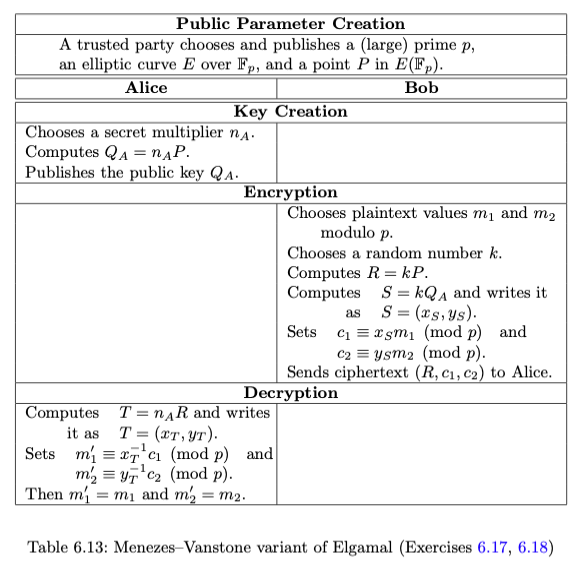
\includegraphics[width=6.5in]{mv-elgamal.png}
		\label{fig:mv}
	\end{figure}
	\end{center}
\end{enumerate}
\end{document}
